\documentclass{article}
\usepackage[a4paper, twoside, hmarginratio={1:1},margin=0cm]{geometry}%% page layout of guide
\usepackage{tikz}
\usetikzlibrary{shapes, shadows}
\begin{document}

\parindent0pt
\null
\colorlet{lessblack}{black!85}
\thispagestyle{empty}

\providecommand{\theguideversion}{1.46p}

\def\nodeshadowed[#1]#2;{%
    \node[scale=1,above,#1]{#2};
    \node[scale=1,above,#1,yscale=-1,scope fading=south,opacity=0.4]{#2};
}%


\begin{tikzpicture}[overlay]
    \coordinate (front) at (0,0);
    \coordinate (top) at (0,1cm);
    \coordinate (bottom) at (0,-\paperheight);
    \coordinate (left) at (0,0);
    \coordinate (right) at (\paperwidth,0);
    \shade [bottom color=white!10,top color=black!35] (bottom -|  left) rectangle (top -| right);
    %\shade [top color=yellow!10,bottom color=yellow!50!brown!90] (bottom -|  left) rectangle (top -| right);
\end{tikzpicture}

\begin{tikzpicture}[remember picture, overlay]
    \node[inner sep=0pt] at (2.5,-19.76) {
        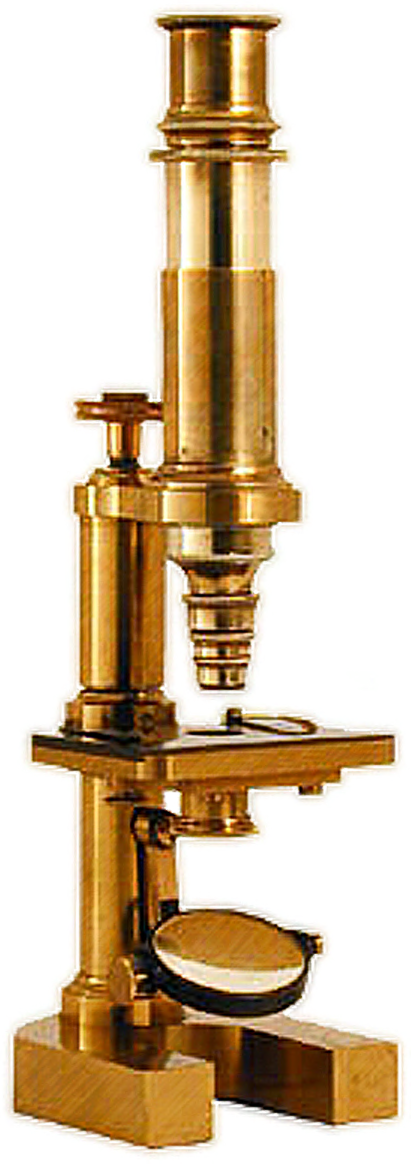
\includegraphics[]{CoverImg.pdf}
    };%
\end{tikzpicture}

\begin{tikzpicture}[overlay]
    \nodeshadowed[scale=3,above,at={(4.5,-22)}, yslant=0] {
        \begin{minipage}{.5\paperwidth}
            \flushright
            \Huge\textcolor{lessblack}{\textbf{ImageJ\\ User Guide}}
        \end{minipage}%
    };%
\end{tikzpicture}

\begin{tikzpicture}[overlay, transform shape, rotate=-45]
    \node[scale=2,above,at={(13.38,9.5)}, yslant=0, fill=orange!50, draw=orange!100, very thick,minimum size=1.6cm] {
        \Huge\textcolor{lessblack}{\textbf{\qquad IJ\,\theguideversion \qquad{}}}
    };%
\end{tikzpicture}

\begin{tikzpicture}[overlay, transform shape, rotate=0]
    \node[scale=1,above,at={(15.1,-.818\paperheight)}, yslant=0] {
        \begin{minipage}{.5\paperwidth}
            \flushright \huge \textcolor{black!90}{\textsc{ImageJ/Fiji\,1.46}}
        \end{minipage}
    };%
\end{tikzpicture}

\end{document}